\documentclass[a4paper, 12pt, oneside]{article}

\usepackage[utf8]{inputenc}
\usepackage[T1]{fontenc}
\usepackage[french]{babel}
\usepackage{array}
\usepackage{shortvrb}
\usepackage{listings}
\usepackage[fleqn]{amsmath}
\usepackage{amsfonts}
\usepackage{fullpage}
\usepackage{enumerate}
\usepackage{graphicx}
\usepackage{subfigure}
\usepackage{alltt}
\usepackage{url}
\usepackage{indentfirst}
\usepackage{eurosym}
\usepackage{listings}
\usepackage{titlesec, blindtext, color}
\usepackage[table,xcdraw,dvipsnames]{xcolor}
\usepackage[unicode]{hyperref}
\usepackage{url}
\usepackage{float}

\definecolor{mygray}{rgb}{0.5,0.5,0.5}

\lstset{
    language=C, % Utilisation du langage C
    commentstyle={\color{MidnightBlue}}, % Couleur des commentaires
    frame=single, % Entoure le code d'un joli cadre
    rulecolor=\color{black}, % Couleur de la ligne qui forme le cadre
    stringstyle=\color{RawSienna}, % Couleur des chaines de caractères
    numbers=left, % Ajoute une numérotation des lignes à gauche
    numbersep=5pt, % Distance entre les numérots de lignes et le code
    numberstyle=\tiny\color{mygray}, % Couleur des numéros de lignes
    basicstyle=\tt\footnotesize, 
    tabsize=3, % Largeur des tabulations par défaut
    keywordstyle=\tt\bf\footnotesize\color{Sepia}, % Style des mots-clés
    extendedchars=true, 
    captionpos=b, % sets the caption-position to bottom
    texcl=true, % Commentaires sur une ligne interprétés en Latex
    showstringspaces=false, % Ne montre pas les espace dans les chaines de caractères
    escapeinside={(>}{<)}, % Permet de mettre du latex entre des <( et )>.
    inputencoding=utf8,
    literate=
  {á}{{\'a}}1 {é}{{\'e}}1 {í}{{\'i}}1 {ó}{{\'o}}1 {ú}{{\'u}}1
  {Á}{{\'A}}1 {É}{{\'E}}1 {Í}{{\'I}}1 {Ó}{{\'O}}1 {Ú}{{\'U}}1
  {à}{{\`a}}1 {è}{{\`e}}1 {ì}{{\`i}}1 {ò}{{\`o}}1 {ù}{{\`u}}1
  {À}{{\`A}}1 {È}{{\`E}}1 {Ì}{{\`I}}1 {Ò}{{\`O}}1 {Ù}{{\`U}}1
  {ä}{{\"a}}1 {ë}{{\"e}}1 {ï}{{\"i}}1 {ö}{{\"o}}1 {ü}{{\"u}}1
  {Ä}{{\"A}}1 {Ë}{{\"E}}1 {Ï}{{\"I}}1 {Ö}{{\"O}}1 {Ü}{{\"U}}1
  {â}{{\^a}}1 {ê}{{\^e}}1 {î}{{\^i}}1 {ô}{{\^o}}1 {û}{{\^u}}1
  {Â}{{\^A}}1 {Ê}{{\^E}}1 {Î}{{\^I}}1 {Ô}{{\^O}}1 {Û}{{\^U}}1
  {œ}{{\oe}}1 {Œ}{{\OE}}1 {æ}{{\ae}}1 {Æ}{{\AE}}1 {ß}{{\ss}}1
  {ű}{{\H{u}}}1 {Ű}{{\H{U}}}1 {ő}{{\H{o}}}1 {Ő}{{\H{O}}}1
  {ç}{{\c c}}1 {Ç}{{\c C}}1 {ø}{{\o}}1 {å}{{\r a}}1 {Å}{{\r A}}1
  {€}{{\euro}}1 {£}{{\pounds}}1 {«}{{\guillemotleft}}1
  {»}{{\guillemotright}}1 {ñ}{{\~n}}1 {Ñ}{{\~N}}1 {¿}{{?`}}1
}

%%%% Page de garde %%%%

\title{\textbf{Introduction aux processus stochastiques}\\
	   Projet 1 : Analyse de propagation d'un virus dans un réseau}
\author{Maxime GOFFART \\180521 \and Olivier JORIS\\182113}
\date{Année académique 2019 - 2020}

\begin{document}

\maketitle
\newpage

\tableofcontents
\newpage

\section{Introduction}

\paragraph{}Les processus stochastiques permettent d'étudier des phénomènes aléatoires dans divers secteurs : l'économie, la climatologie, la météorologie, la biologie, \dotso

\paragraph{}En particulier dans ce projet, il nous a été demandé d'étudier un phénomène d'actualité : la propagation d'un virus au sein d'un réseau, pouvant peut être modélisé à l'aide d'une chaîne de Markov. Ainsi, ce projet nous a permis d'appliquer les concepts vus au cours sur un exemple concret et d'actualité.

\section{Structure du programme} 
\paragraph{}Je (max) le ferais plus tard tkt.

\section{Etude du modèle exact}

\subsection{Question 1}
	
\paragraph{}Le modèle proposé dans l'énoncé est bien un processus de Markov en temps discret caractérisé par ses $3^N$ états \footnote{$N$ étant la taille de la population.}. Les états de cette chaînes sont caractérisés par la suite de longueur $N$ des catégories \footnote{S, R ou I.} auxquelles appartiennent les individus \footnote{Les individus étant indexés de 1 à N.} à l'instant t. Par exemple : pour $N = 3$, l'état "'S' 'I' 'I'" représente le fait que le premier individu est susceptible d'être infecté et que les deux derniers sont infectés.\\
\indent Les probabilités de transitions d'un état à un potentiel état de l'instant suivant de la chaîne dépendent à la fois de chacune des catégories des individus à l'instant initial et de leurs interactions avec des personnes infectées \footnote{Modélisées par le graphe $W$.}.\\
\indent Les états de cette chaîne qui sont uniquement composés d'individus de la catégorie 'R' ou\footnote{Il s'agit d'un "ou" inclusif.} de la catégorie 'S' sont absorbants car la propagation du virus n'est plus possible s'il n'y a plus d'infectés. Il en va de même pour les états dans lesquels les infectés n'ont de contact avec personne\footnote{Cela correspond à une ligne remplie de 0 dans le graphe $W$.}. Cette chaîne n'est donc ni irréductible, ni régulière, ni périodique.

\subsection{Question 2}

\paragraph{}Il faudra en moyenne ... à un individu pour guérir une fois infecté.

\subsection{Question 3}

\paragraph{}Pour répondre à cette question, le programme peut-être lancé à l'aide de la commande suivante :

\begin{lstlisting}[language=bash]
$ python3 exact_model.py matrixSize fileName
\end{lstlisting}

\noindent où la première option spécifie la taille de la matrice $W$ utilisée et la deuxième représente le nom du fichier dans lequel cette matrice est encodée. Ensuite, le programme demande à l'utilisateur sur combien de simulations celui-ci veut que les calculs soient effectués pour la génération du graphique.

\paragraph{}Ainsi, en lançant le programme avec cette commande :

\begin{lstlisting}[language=bash]
$ python3 exact_model.py 6 6x6_lin.txt
\end{lstlisting}

\noindent On obtient le graphique de la figure 1 répondant à la première partie de la question avec les paramètres $\mu$ et $\beta$ fixés aux valeurs suggérées.

\begin{figure}[H]
	\centering
	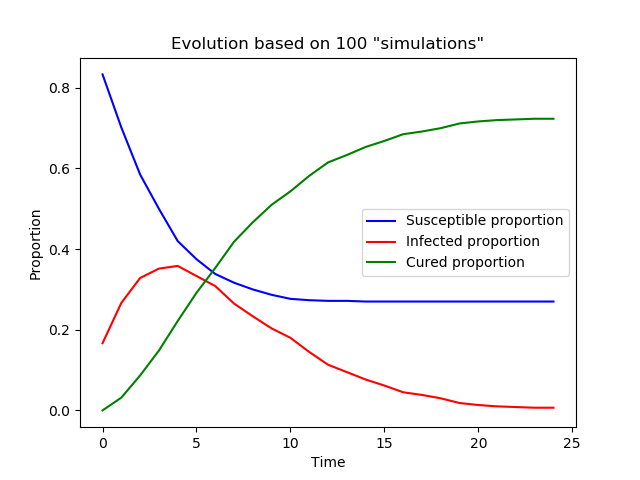
\includegraphics[scale=1]{lin_6x6.png} 
	\caption{Evolution des proportions d'individus dans chacune des catégorie au cours du temps suivant un modèle représenté par une matrice $W_{lin}$.}
\end{figure}

\paragraph{}Sur la figure 1, on observe le fait que la proportion d'individus infectés est décroissante. En effet, les individus ayant peu de contacts les uns avec les autres, la probabilité qu'un individu soit infecté est faible. De plus, les individus initialement infectés finissent par guérir. On observe, également, qu'une partie de la population reste "susceptible" d'obtenir le virus car elle ne l'a jamais contracté car les relations entre les individus sont limitées.

\paragraph{}De la même façon en lançant le programme à l'aide de cette commande :
\begin{lstlisting}[language=bash]
$ python3 exact_model.py 6 6x6_full.txt
\end{lstlisting}

\noindent On obtient le graphique de la figure 2 répondant à la deuxième partie de la question avec les paramètres $\mu$ et $\beta$ fixés aux valeurs suggérées.

\begin{figure}[H]
	\centering
	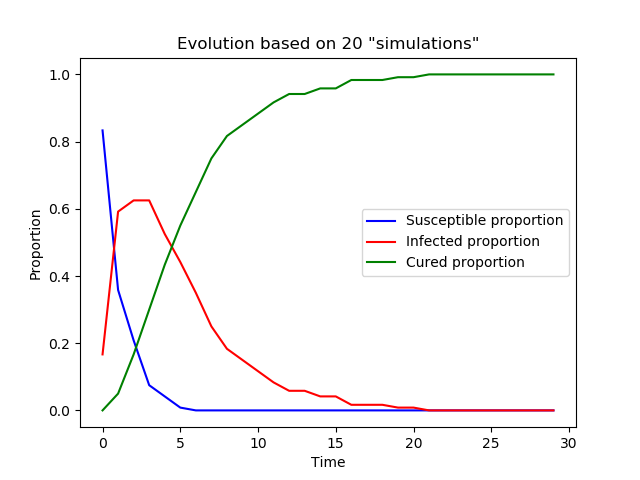
\includegraphics[scale=1]{full_6x6.png} 
	\caption{Evolution des proportions d'individus dans chacune des catégorie au cours du temps suivant un modèle représenté par une matrice $W_{full}$.}
\end{figure}

\paragraph{}Sur la figure 2, on observe, à l'inverse de la situation précédente, que la population connaît un nombre important d'infectés et très rapidement car les gens sont tous en contact. Au temps t = 25, on peut voir que la proportion d'individus susceptibles est proche de 0, c'est-à-dire que presque toute la population a été infecté à un instant inférieur ou égal à celui-ci. En effet, les individus ayant tous des contacts les uns avec les autres, le virus ne fait que se propager au sein de la population jusqu'à ce que celle-ci soit entièrement guérie.

\subsection{Question 4}

\paragraph{}Lors de l'exécution des deux précédentes commandes, le programme nous retourne également le temps moyen nécessaire à la disparition du virus dans la population. Nous avons obtenus une moyenne de 11,56 dans le cas où les contacts entre les gens sont limités\footnote{Celui qui utilise la matrice $W_{lin}$.} et une moyenne de 14,48 dans l'autre cas\footnote{Celui qui utilise la matrice $W_{full}$.}.
\paragraph{}On observe que le premier modèle\footnote{Celui dont la matrice d'adjacence est $W_{lin}$.} nécessite un temps inférieur au second avant d'atteindre une situation stable. Ceci s'explique par le fait que le virus se répand mois rapidement\footnote{Car les gens sont moins en contact les uns avec les autres.} donc les gens qui sont infectés transmettent le virus à moins d'individus donc la proportion de personnes infectés est plus rapidement sous contrôle. Comme mentionné précédemment, une partie de la population n'est pas infectée par les virus donc il n'est pas nécessaire de les soigner ce qui permet de gagner du temps.
\paragraph{}A l'inverse, dans le deuxième cas\footnote{Celui dont la matrice d'adjacence est $W_{full}$.}, le temps avant la disparition du virus est plus long car une grande majorité de la population est rapidement atteinte donc le seul moyen d'arriver à une situation "stable" est de soigner tout le monde. Dans le cas de la question 3, la probabilité d'être guéri est donné par $\mu = 0,2$ donc le temps nécessaire pour avoir une population entièrement guérie est long.

\section{Etude sur base de simulations}

\subsection{Question 1}

\paragraph{}L'hypothèse d'indépendance posée par les auteurs de l'article n'est en général pas vérfiée car la probabilité qu'un individu se trouve dans un état à un instant \textit{t} dépend en partie de son interaction avec les autres personnes de la population et de leur état à un instant précédent. Ainsi, si un individu dans un état \textit{susceptible} a des contacts avec des individus dans un état \textit{infectieux}, alors son état à un instant $t' > t$ sera impacté par ces derniers. L'indépendance n'est donc vérifiée que dans le cas où un individu n'a de contact avec personne.

\subsection{Question 2}

\paragraph{}Pour répondre à cette question, le programme peut-être lancé à l'aide de la commande suivante :
\begin{lstlisting}[language=bash]
$ python3 simulations_study.py populationSize fileName 
\end{lstlisting}
\noindent où la première option spécifie la taille de la matrice $W$ utilisée et la deuxième option correspond au nom du fichier dans lequel cette matrice est encodée.

\paragraph{}Ainsi, en lançant le programme avec cette commande :

\begin{lstlisting}[language=bash]
$ python3 simulations_study.py 6 6x6_lin.txt 
\end{lstlisting}

\noindent Le programme demande à l'utilisateur les paramètres que celui-ci souhaite utiliser pour les simulations. Ensuite, le script retourne le graphique de la figure 3 ainsi que le temps moyen de disparition des individus infectieux y correspondant. On observe ainsi que l'étude sur base du modèle exact et celle sur base de simulations coïncident pour le cas où la matrice d'adjacence correspond à $W_{lin}$.

\begin{figure}[H]
	\centering
	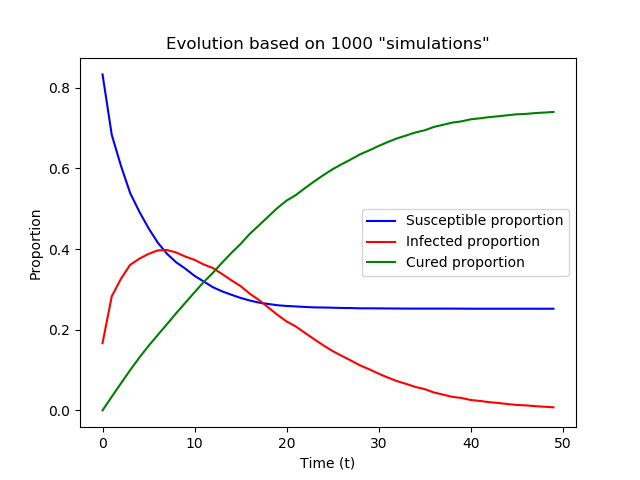
\includegraphics[scale=1]{lin_6x6_simulations.png} 
	\caption{Evolution des proportions d'individus dans chacune des catégories au cours du temps suivant un modèle représenté par une matrice $W_{lin}$ de taille $6 \times 6$.}
\end{figure}

\paragraph{}De la même façon en lançant le programme à l'aide de cette commande\footnote{Et en choisissant d'utiliser 10 simulations.}:
\begin{lstlisting}[language=bash]
$ python3 simulations_study.py 6 6x6_full.txt 
\end{lstlisting}

\noindent On obtient le graphique de la figure 4 ainsi que le temps moyen de disparition des individus infectieux y correspondant avec les probabilités $\beta$ et $\mu$ fixées au valeurs suggérées. On observe que l'étude sur base du modèle exact et celle sur base de simulations coïncident également dans ce cas de figure. On peut donc penser que cette simulation approxime de manière satisfaisante la réalité et permettrait ainsi de modéliser cette même simulation avec une population plus nombreuse\footnote{En prenant un nombre de simulations suffisamment pour que les calculs soient stables}.

\begin{figure}[H]
	\centering
	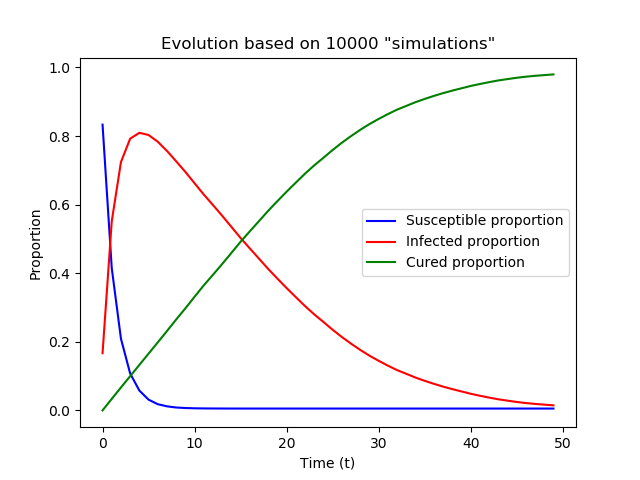
\includegraphics[scale=1]{full_6x6_simulations.png} 
	\caption{Evolution des proportions d'individus dans chacune des catégorie au cours du temps suivant un modèle représenté par une matrice $W_{full}$ de taille $6 \times 6$.}
\end{figure}

\subsection{Question 3}

\paragraph{}En lançant le programme à l'aide de la commande suivante\footnote{Et en choisissant un nombre suffisant de simulations pour avoir des résultats stables.} 

\begin{lstlisting}[language=bash]
$ python3 simulations_study.py 2000 Wbig_dense.txt 
\end{lstlisting}

\noindent Le programme retourne le graphique de la figure 5 ainsi que le temps moyen de disparition des individus infectieux y correspondant avec les probabilités $\beta$ et $\mu$ fixées au valeurs suggérées.

\begin{figure}[H]
	\centering
	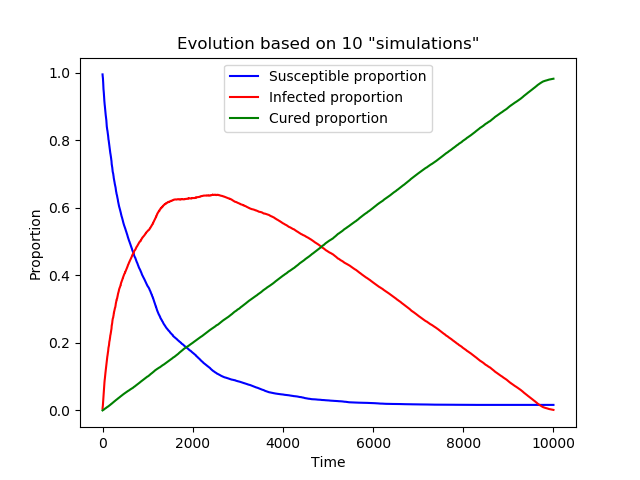
\includegraphics[scale=1]{Wbig_dense_simulations.png} 
	\caption{Evolution des proportions d'individus dans chacune des catégorie au cours du temps suivant un modèle représenté par une matrice d'adjacence $W_{big}$ de taille $2000 \times 2000$ générée aléatoirement selon un modèle "scale-free" avec aucune mesure n'est prise.}
\end{figure}

\subsection{Question 4}

\paragraph{}Si le graphique de la figure 5 représente l'évolution de l'épidémie dans le cas où aucune mesure n'est prise. Etudions l'impact des mesures suivantes :

\paragraph{}(a) Réduire la probabilité de transmission de la maladie via différents moyens revient à diminuer la probabilité de contamination $\beta$. Ainsi, en réduisant la probabilité $\beta$ à 0.2, on obtient le graphique de la figure 6 qui permet de visualiser que cette mesure permet d'avoir une proportion de la population qui ne voit pas infecter par le virus. De plus, le temps de disparition de ce dernier se voit diminuer\footnote{Valant ici environ 8300}.

\begin{figure}[H]
	\centering
	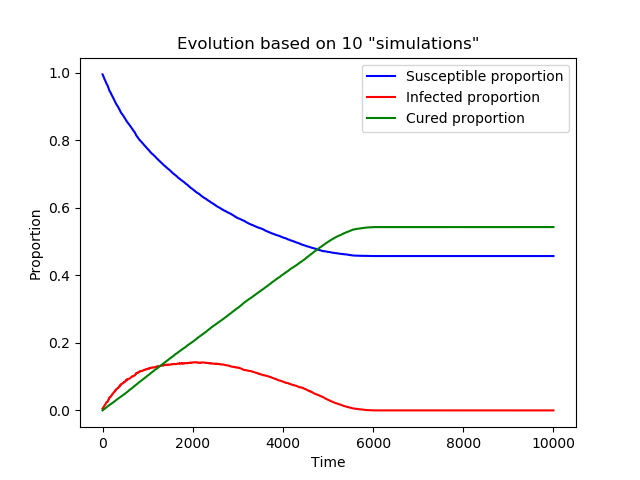
\includegraphics[scale=1]{Wbig_dense_reduction_transmission.png} 
	\caption{Evolution des proportions d'individus dans chacune des catégorie au cours du temps suivant un modèle représenté par une matrice d'adjacence $W_{big}$ de taille $2000 \times 2000$ générée aléatoirement selon un modèle "scale-free" avec une probabilité de transmission réduite.}
\end{figure}


\paragraph{}(b) Réduire les interactions entre les individus revient à diminuer le nombre de 1 dans la matrice $W$. 

\paragraph{}(c) Vacciner un certain pourcentage de la population correspond à ajouter cette proportion d'individus dans l'état 'R' à l'instant $t = 0$. Le graphique de la figure 8 représente la situation où 30\% de la population est vaccinée. Celui-ci permet également d'avoir une proportion d'individus qui n'est jamais infectée et de réduire le temps de disparition du virus\footnote{Valant ici environ 6000}.

\begin{figure}[H]
	\centering
	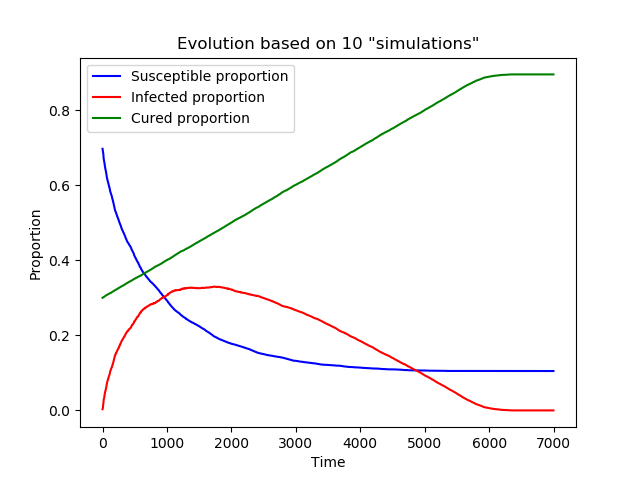
\includegraphics[scale=1]{Wbig_dense_initial_immunised.png} 
	\caption{Evolution des proportions d'individus dans chacune des catégorie au cours du temps suivant un modèle représenté par une matrice d'adjacence $W_{big}$ de taille $2000 \times 2000$ générée aléatoirement selon un modèle "scale-free" avec une proportion d'individus vaccinés.}
\end{figure}

\paragraph{}(d) Traiter les patients avec un médicament qui permettrait d'accélérer la guérison revient à augmenter la probabilité de guérison $\mu$. En augmentant la probabilité de guérison à 0.5, on voit que la principale amélioration est la vitesse de disparition du virus\footnote{Passant ici à environ 3600}. On voit également qu'une proportion d'individu ne se fait pas infecter.

\begin{figure}[H]
	\centering
	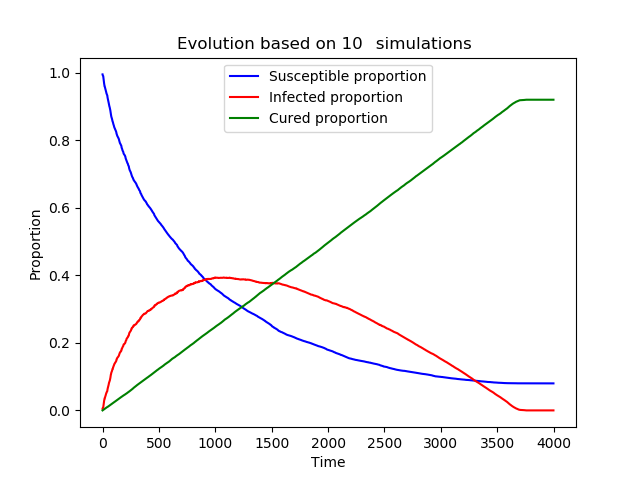
\includegraphics[scale=1]{Wbig_dense_speeded_heal.png} 
	\caption{Evolution des proportions d'individus dans chacune des catégorie au cours du temps suivant un modèle représenté par une matrice d'adjacence $W_{big}$ de taille $2000 \times 2000$ générée aléatoirement selon un modèle "scale-free" avec une proportion d'individus vaccinés.}
\end{figure}

\subsubsection{Comparaison des différentes mesures}

\end{document}